\documentclass{beamer}
\usetheme{Antibes}
\usecolortheme{seahorse}
\setbeamertemplate{itemize items}[default]

\title{Django-Style Flask}
\author[Cody Lee]{Cody Lee\linebreak \texttt{codylee@wellaware.us}\linebreak
\footnotesize
git clone \url{https://github.com/platinummonkey/flask\_scale12x.git}}
\date{SCALE12x

Feb 22, 2014}

\begin{document}

\begin{frame}
\titlepage
\end{frame}

\frame{
\begin{center}

\includegraphics[width=5cm]{images/FairWarning.jpg}

\includegraphics[width=5cm]{images/picard_do_it_live.jpg}
\end{center}
}

\frame{
\frametitle{Introduction}
\begin{itemize}
\item Senior Network Engineer at WellAware - An oil and gas SaaS and network communications company
\item Conference Chairman for the annual Texas Linux Festival
\begin{itemize}
\item Come check us out June 13-14 in Austin, TX!
\item \url{http://texaslinuxfest.org} for more information
\end{itemize}
\item Yes, I'm really a Mechanical Engineer
\begin{itemize}
\item Bachelors of Science in Mechanical Engineering at Texas A\&M University
\item Master's student at University of Texas at San Antonio
\end{itemize}
\end{itemize}
}

\frame{
\frametitle{Outline}
\begin{columns}
\begin{column}{5cm}
\tableofcontents
\end{column}
\begin{column}{4cm}
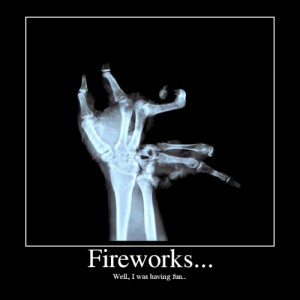
\includegraphics[width=5cm]{images/fireworks.jpg}
\end{column}
\end{columns}
}

\section{Get Prepared}
\begin{frame}[fragile]
\frametitle{Get Prepared}
\begin{itemize}
\item \footnotesize git clone \url{https://github.com/platinummonkey/flask\_scale12x.git}\normalsize
\item Run the \emph{viewer\_setup.sh} script to setup the helper scripts.
\item (Optional*) Setup and Start Titan: run \emph{setup\_titan.sh} and \emph{start\_titan.sh}.
\item (Optional*) Setup virtualenv:
\begin{verbatim}
mkvirtualenv -a <repo_root> \
    -r <repo_root>/requirements.pip \
    flask_scale12x
\end{verbatim}
\item Utilize \emph{talk\_helper.sh} during the talk to switch between commits easily.
\end{itemize}
\end{frame}

\section{Flask and Django}
\subsection{Django}
\frame{
\frametitle{Django}
\begin{itemize}
\item "Batteries Included" \linebreak
\begin{center}

\includegraphics[width=2cm]{images/batteries_included.jpg}
\end{center}
\item Early Framework led to early adoption \linebreak
\begin{center}
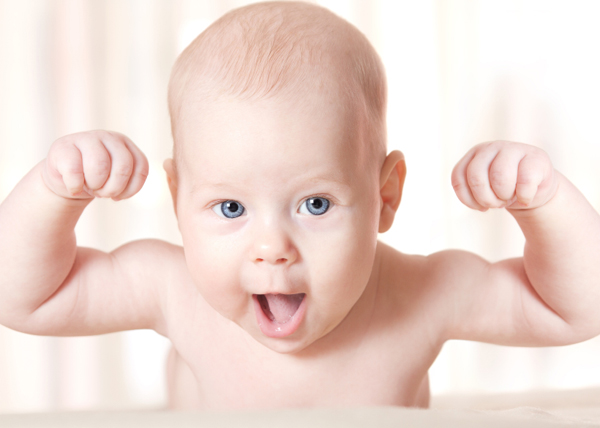
\includegraphics[width=4cm]{images/baby-surprise.jpg}
\end{center}
\end{itemize}
}

\frame{
\frametitle{Django}
\begin{columns}
\column{1.0\textwidth}
\begin{itemize}
\item Monolithic approach
  \begin{itemize}
  \item Organization - Everything is an app
  \item Url importing and view routing
  \item Models - ORM with DB Managers for use with RDBs
  \item Admin
  \item Builtins
    \begin{itemize}
    \item Auth \& Permissions
    \item Testing
    \item Configuration
    \end{itemize}
  \end{itemize}
\end{itemize}
\column{0.1\textwidth}
\hspace*{-1.5cm}
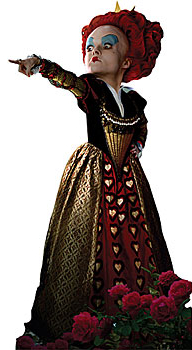
\includegraphics[width=3.5cm]{images/red-queen.jpg}
\end{columns}
}

\frame{
\frametitle{Django}
\begin{columns}[T]
\column{0.99\textwidth}
\begin{itemize}
\item Documentation
\item Templating
\item Extensions
\item Django-NoSQL project
  \begin{itemize}
  \item For use with NoSQL DBs [however its just an adapter]
  \end{itemize}
\end{itemize}
\column{0.01\textwidth}
\hspace*{-2.5cm}

\includegraphics[width=3cm]{images/document_all_things.jpg}
\end{columns}
}

\subsection{Flask}
\frame{
\frametitle{Flask}
\begin{itemize}
\item Flexible by Design
\begin{center}
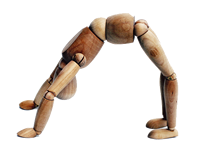
\includegraphics[width=3cm]{images/flexible.png}
\end{center}
\item No forced organization pattern
\begin{center}

\includegraphics[width=3cm]{images/guy-fawkes.jpg}
\end{center}
\item URL routing happens at the View Definition
\end{itemize}
}

\frame{
\frametitle{Flask}
\begin{columns}[T]
\column{0.99\textwidth}
\begin{itemize}
\item Documentation
  \begin{itemize}
  \item Great but could be better
  \item Version docs are not separated
  \item Changes noted explicitly within the \emph{latest} docs.
  \end{itemize}
\item Templating
  \begin{itemize}
  \item Request object is implicitly context aware
  \item Jinja2
    \begin{itemize}
    \item Done right - Doesn't unecessarily limit programmer
    \item Run python code and use callables
    \end{itemize}
  \end{itemize}
\end{itemize}
\column{0.01\textwidth}
\hspace*{-2.5cm}

\includegraphics[width=3cm]{images/scattered_docs.jpg} 
\column{0.01\textwidth}
\vspace*{2cm}
\hspace*{-2cm}

\includegraphics[width=2cm]{images/jinja-small.png}
\end{columns}
}

\frame{
\frametitle{Flask}
\begin{columns}
\column{0.99\textwidth}
\begin{itemize}
\item Extensions
  \begin{itemize}
  \item Auth - Flask-Login
  \item Permissions - Flask-Principal (if simple enough)
  \item Configuration - Flask-Environment
  \item Testing - Flask-Testing
  \end{itemize}
\end{itemize}
\column{0.01\textwidth}
\hspace*{-2cm}

\includegraphics[width=2cm]{images/puzzle.png}
\end{columns}
}


\subsection{Side-By-Side}
\begin{frame}
\frametitle{Flask and Django Side-by-Side}
\begin{columns}
  \begin{column}[T]{5cm}
  Django
  
  \begin{itemize}
    \item "Batteries Included"
    \item Forced Organization Pattern
    \item Monolithic approach
    \item Url importing and view routing
    \item ORM
    \item Many Builtins
    \item Great Documentation
    \item Okay Templating
    \item Extensions available
  \end{itemize}
  \end{column}
  
  \begin{column}[T]{5cm}
  Flask
  
  \begin{itemize}
    \item No Batteries
    \item No forced organization pattern
    \item Modular approach
    \item URL routing happens at the View Definition
    \item No ORM forced
    \item Minimal Builtins
    \item Good Documentation
    \item Better Templating
    \item Extensions usually required
    \end{itemize}  
  \end{column}
\end{columns}
\end{frame}

\section{Django Sugar}
\subsection{What We Care About}
\frame{
\frametitle{Django Sugar}
\begin{columns}
\begin{column}{8cm}
What was really nice to have?

\begin{itemize}
\item Organization
\item Global Application Context
\item Configuration
\item URL and View Routing
\item ORM \& Models
\item Auth \& Sessions
\item Testing
\item Permissions
\end{itemize}
\end{column}

\begin{column}{3cm}
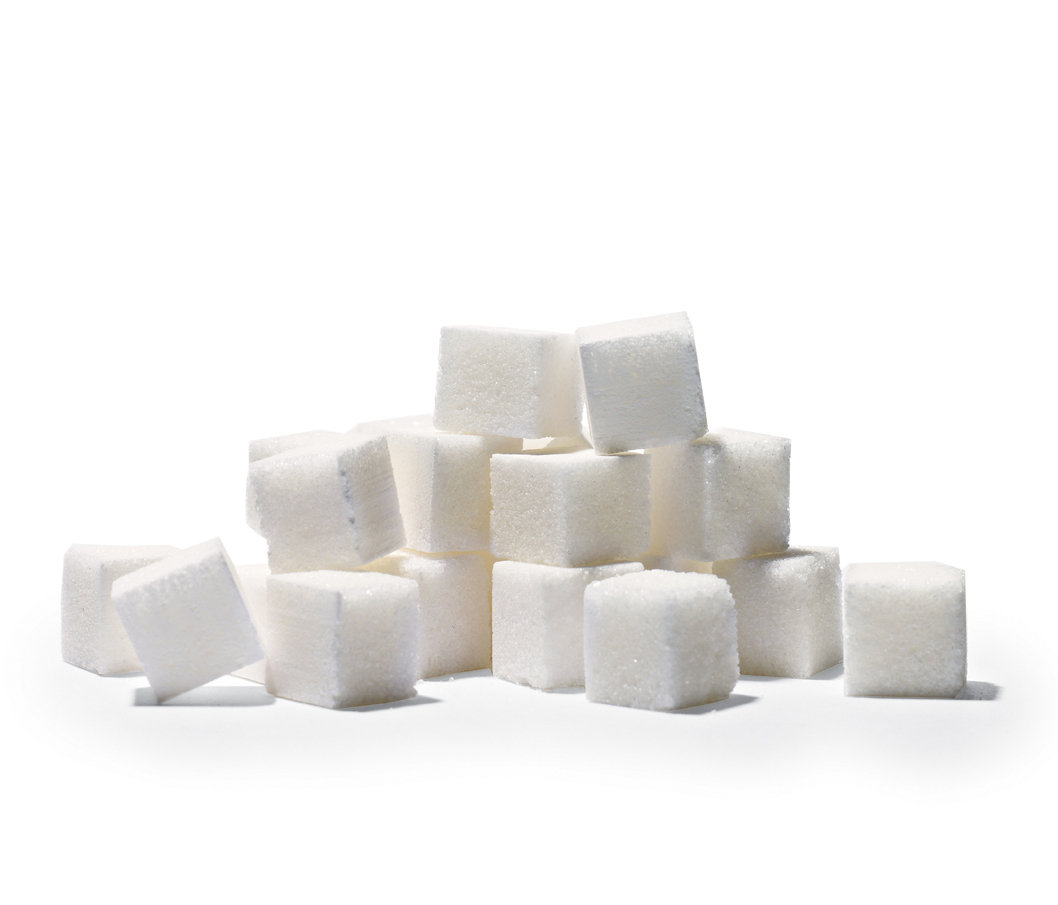
\includegraphics[width=3cm]{images/sugar_cubes.jpg}
\end{column}
\end{columns}
}

\subsection{Sugar Cube}
\begin{frame}
\frametitle{Organization}
\begin{block}{This where you get to decide how everything gets laid out!}
Let's just go with Django's "everything is an app" approach for this context. Feel free to do anything sensible (or not).
\end{block}
\tiny
\emph{\textless project\_root\textgreater}
\begin{itemize}
\item app.py, models.py, requirements.pip, server.py, shell.py, urls.py, version.py, views.py
\item auth
  \begin{itemize}
  \tiny
  \item \_\_init\_\_.py, decorators.py, models.py, urls.py, views.py
  \item permissions
    \begin{itemize}
    \tiny
    \item \_\_init\_\_.py, decorators.py, permissions.py
    \end{itemize}
  \item tests...
  \end{itemize}
  \tiny
\item config
  \begin{itemize}
  \tiny
  \item \_\_init\_\_.py, base.py, development.py, production.py, staging.py
  \end{itemize}
\item tools
  \begin{itemize}
  \tiny
  \item apps.py, constants.py, login\_manager.py, url\_tools.py, sessions.py, ...
  \end{itemize}
\end{itemize}
\normalsize
\end{frame}


\frame{
\frametitle{Global Application Context}
\begin{itemize}
\item The main \emph{app.py}!
\linebreak
\begin{center}
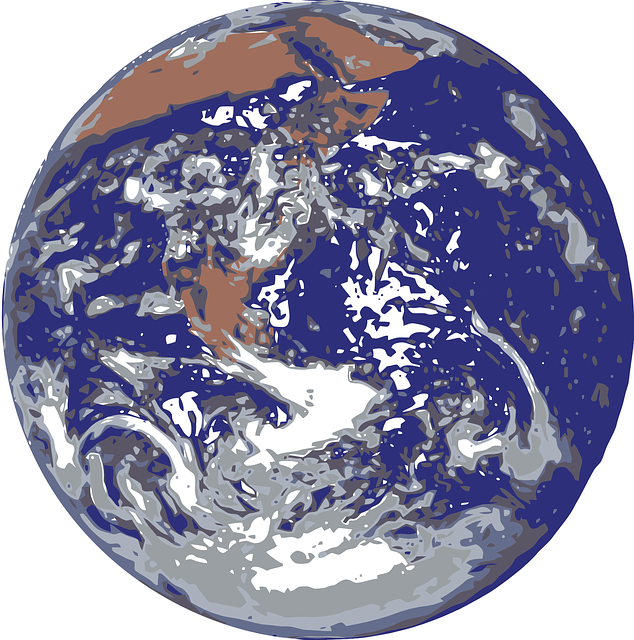
\includegraphics[width=2cm]{images/earth.png}
\end{center}
\item Pretty common method, with a very slight twist
\item TO THE CODE! \linebreak \emph{683e32dd75361d4f87687b4f2235de8af455b950}
\end{itemize}
}

\frame{
\frametitle{Configuration}
\begin{itemize}
\item Flask-Environments
\item Utilize FLASK\_ENVIRONMENT environment variable
\item TO THE CODE! \linebreak \emph{028b31d21435954cb2579a6e780d579f6d599c00}
\end{itemize}
\begin{center}
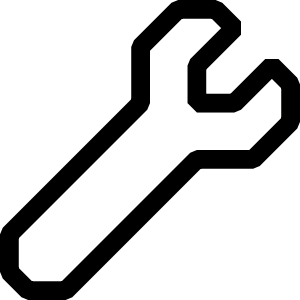
\includegraphics[width=3cm]{images/wrench.png}
\end{center}
}

\frame{
\frametitle{URL and View Routing}
\begin{itemize}
\item Here is where things get sugary.
\item How does Django do it? How do we want it?
  \begin{itemize}
  \item \emph{INSTALLED\_APPS}
  \item tooling
  \end{itemize}
\item TO THE CODE! \linebreak \emph{ba95b15727bd4f543e907e4e12d06112d750168f}
\end{itemize}
\begin{center}

\includegraphics[width=3cm]{images/ermahgerd-aliens.jpg}
\end{center}
}

\frame{
\frametitle{ORM \& Models}
\begin{columns}[T]
\column{1.05\textwidth}
\begin{itemize}
\item Pick a Database (SQL, NoSQL, Graph, Key-Value, ...)
\item Hope that it has a sane ORM, if not...
\item CREATE ONE!
\item We'll use bulbs (a really cool OGM) and factory\_boy
\item How do we want to integrate it! Just the same way! Utilize INSTALLED\_APPS loader
\item TO THE CODE! \linebreak
\emph{a3ca56d346731b9ca953f0c08fda3fb99325d353}
\end{itemize}
\column{0.01\textwidth}
\hspace*{-2cm}

\includegraphics[width=2cm]{images/challenge_accepted.png}
\end{columns}
}

\frame{
\frametitle{Auth \& Sessions}
\begin{itemize}
\item Auth and sessions are built-in to Django, not so much in Flask
\item Create or own \emph{auth app} and models
\item Implement Authentication with Flask-Login and Flask-Cache!
\item TO THE CODE! \linebreak
\emph{66c2c5b14e52584892d1a28a9dd33f112d57591c}
\end{itemize}
\begin{center}
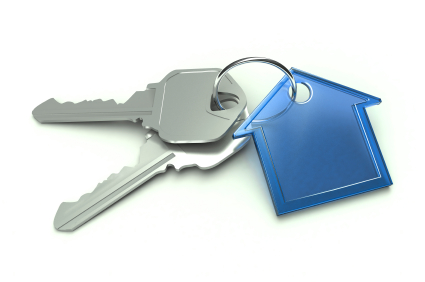
\includegraphics[width=3cm]{images/authentication.jpg}
\end{center}
}


\frame{
\frametitle{Testing}
\begin{itemize}
\item Django has a TestRunner built-in - creates test database and... Flask doesn't
\item We still have nose!
\item We also have Flask-Testing!
\item TO THE CODE! \linebreak
\emph{66c2c5b14e52584892d1a28a9dd33f112d57591c}
\end{itemize}
\begin{center}
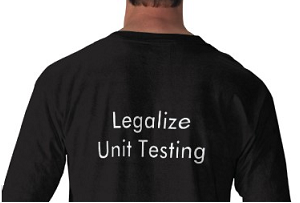
\includegraphics[width=5cm]{images/unit-testing.png}
\end{center}
}

\frame{
\frametitle{Permissions}
\begin{itemize}
\item Permisisons are built-in to Django (Though Guardian is way better)
\item Create our own or use Flask-Prinicpal
\item Preview available in code \linebreak
\emph{66c2c5b14e52584892d1a28a9dd33f112d57591c}
\end{itemize}
\begin{center}

\includegraphics[width=4cm]{images/grumpy_cat.png}
\end{center}
}

\section{Wrap it All Up}
\frame{
\frametitle{Wrapping it All Up}
\begin{columns}
\column{0.99\textwidth}
\begin{itemize}
\item Whoa! This looks and feels \emph{sorta} like Django!
\item What we've done today:
  \begin{itemize}
  \item Organization
  \item Global Application Context
  \item Configuration
  \item URL and View Routing
  \item ORM \& Models
  \item Auth \& Sessions
  \item Testing
  \item Permissions
  \end{itemize}
\end{itemize}
\column{0.01\textwidth}
\hspace*{-2cm}

\includegraphics[width=2cm]{images/mummy.png}
\end{columns}
}

\frame{
\frametitle{So am I using this?}
\begin{center}
No. \linebreak
We're moving off of Django to Falcon. \linebreak \url{http://falconframework.org/}
\linebreak

\includegraphics[width=4cm]{images/falcon_logo.png}
\end{center}
}

\section{Questions}
\frame{
\begin{center}
Questions?

Comments?
\linebreak
\linebreak
\linebreak
\emph{Please just wake up.}
\end{center}
}

\end{document}
